\begin{document}

% self defined colors for colored code (can add more colors)
\definecolor{green}{rgb}{0.1,0.5,0.2} % rgb defined between 0 and 1
\definecolor{blue}{rgb}{0,0.3,0.7}
\definecolor{purple}{rgb}{0.7,0,0.7}
\definecolor{gray}{rgb}{0.5,0.5,0.5}
\definecolor{codeorange}{rgb}{0.9,0.3,0}

% writing code in the document as list
% can be changed, add changed version before your code (possible to have multiple versions within one doc)
\lstset{ 
  basicstyle=\ttfamily\UseRawInputEncoding\small,
  extendedchars=true, % lets you use non-ASCII characters; for 8-bits encodings only, does not work with UTF-8
  breaklines=true,                 
  escapeinside={\%*}{*)}, % if you want to add LaTeX within your code
  keepspaces=true,
  morekeywords={*,...}, % if you want to add more keywords
  showstringspaces=false,          
  tabsize=2, % sets default tabsize to 2 spaces
  numbersep=5pt, % how far the line-numbers are from the code
  numbers=left,                   
  numberstyle=\tiny\color{gray},
  stringstyle=\color{purple},
  commentstyle=\color{gray},
  keywordstyle=\color{blue},
  identifierstyle=\color{codeorange}
}

%=================================================================
%                           Start Document
%=================================================================
\section{Results}
\lhead{Results} % section header

\subsection{Open Loop Stimulation Sequence}

\subsection{Knee Angle Estimation}
Accurate knee angle estimation is critical for the closed loop FES application. Therefore the Madgwick knee angle stimation technique was validated by comparing the IN-House IMU based knee angle estimation with the DELSYS IMU base knee angle estimate as a benchmark. Delsys IMUs provide high-quality orientation data by leveraging advanced sensor fusion algorithms, designed specifically for biomechanical and movement studies \todo{source add more detail}. 

\todo{Picture of setup w delsys}

The method for knee angle estimation using the In-House IMUs is described throroughly in the methdods section "Knee Angle Estimation". The method for extracting the knee angle from the Delsys sensors involved capturing the orientation data that the sensors provide already having used sensor fusion. The relative orientation between the two sensors is then computed by taking the inverse of the thighs sensoræs rotation and applying it to the shank sensoræs rotation. This relative rotation is then converted to Euler angles from which the rotation about the x-axis is extracted:
\begin{equation}
    \theta_{\text{knee}} = \text{Euler}_x \left( \mathbf{q}_{\text{thigh}}^{-1} \otimes \mathbf{q}_{\text{shank}} \right)
\end{equation}

The validation experiment consisted of mounting the Delsys IMUs and In-House IMUs on the thigh and shank as seen in figure \todo{ref}. The subject was then instructed to sit and move their leg from resting on the ground at approximately a 90 degree angle to resting it on a chair at a full extension, meaning approximately zero degrees. In order to compare the two estimates, the computed knee angles were synchonized and compared over a shared time range. Linear interpolation was applied to both datasets to align them temporally, accounting for potential differences in sampling rates and starting times. The synchronized data allows for a direct comparison as can be seen in figure \ref{fig:t11}. 

\begin{figure} [H]
    \centering
    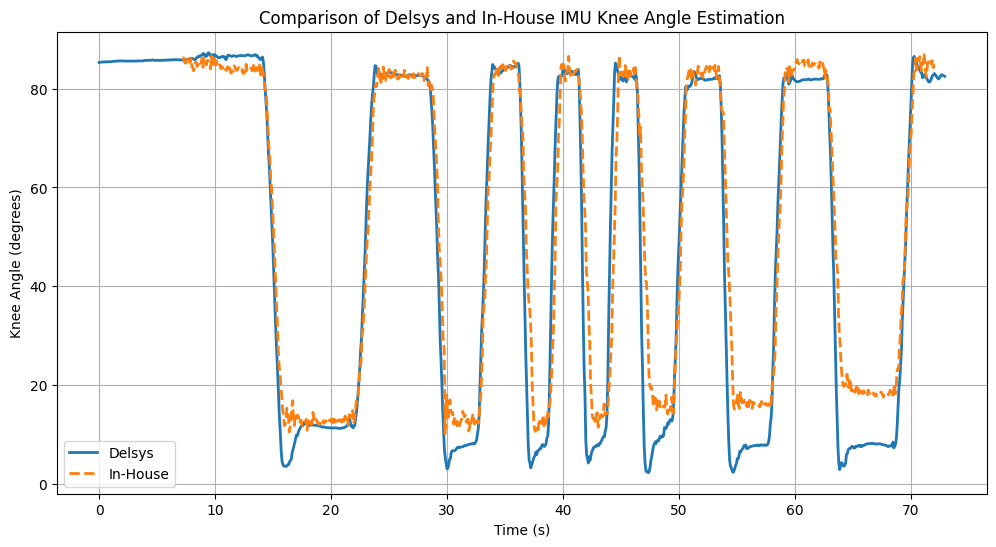
\includegraphics[width=0.95\linewidth]{images/T11_betterplotting.png}
    \caption{}
    \label{fig:t11}
\end{figure}

The results show that the adapted Madgwick filter does a good job of estimating the knee angle. However we see some slight drift, even though the Madgwick filter should in theory be robust to drift. It is however worth noting here that there are some clear inaccuracies in the Delys derived knee angle as well. Specifically we observe that there is a valley in the calculated knee angle followed by a flattening out of the curve when the knee is extended, this does not reflect the actual movement that the subject performs. The ideal performance of the IN-House developed knee angle estimation is therefore not necessarily an exact replication of the Delsys curve. The In-House algorithm does not seem to have this same artifact. 



\subsection{Closed-Loop}

\begin{figure}
    \centering
    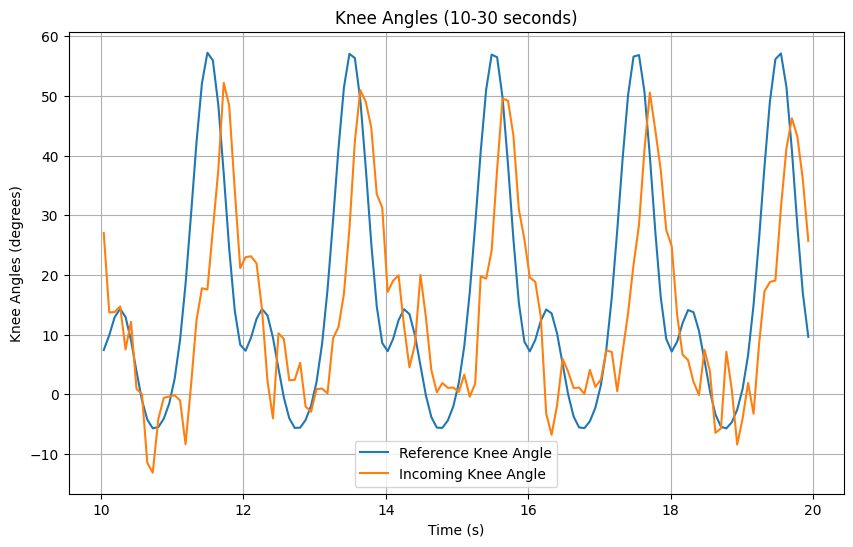
\includegraphics[width=0.5\linewidth]{images/CL12ref.png}
    \caption{Closed loop knee angles}
    \label{fig:el12ref}
\end{figure}


%=================================================================
%                           End Document
%=================================================================
\end{document}